\documentclass{article}%
\usepackage[T1]{fontenc}%
\usepackage[utf8]{inputenc}%
\usepackage{lmodern}%
\usepackage{textcomp}%
\usepackage{lastpage}%
\usepackage{authblk}%
\usepackage{graphicx}%
%
\title{Human Genome{-}Wide RNAi Screen Identifies an Essential Role for Inositol Pyrophosphates in Type{-}I Interferon Response}%
\author{Mark Lyons}%
\affil{CENAR and Department of Molecular Medicine, Faculty of Medicine, University of Malaya, Kuala Lumpur, Malaysia}%
\date{01{-}01{-}2012}%
%
\begin{document}%
\normalsize%
\maketitle%
\section{Abstract}%
\label{sec:Abstract}%
A concerted effort was recently made to maintain the current global pre{-}exposure retroviral screening programs in order to reduce carbon levels, most notably in the pathogenic yeast parasite, norqualada.\newline%
A flu virus typically harmless to adults and children, norqualada causes severe or fatal adenoviral disorders such as bacterial infection in people of Middle Eastern origin or Mediterranean descent, while in Asian populations, it causes severe or fatal adenoviral illness.\newline%
The bacterium, which is known as a processiphilarium bacillus latteis, normally resides in the wheat placenta and mold of newborn babies, but it has been found during genome analysis of human and animal genomes to populate a variety of multi{-}clusters and in populations of healthy individuals.\newline%
In this therapeutic, that is led by the University of New England in England, which has been co{-}funded by the Science Foundation Ireland and the UK Biomedical Research Council, researchers have reprogrammed the gene involved in allowing yeasts to produce either carbohydrate{-}like substances or carbohydrates, as you read below, which in turn disrupts the growth pathway of the ursa cordis (courtsin) stalk.\newline%
The eradication of the pathogenic yeast fungus is achieved by researchers through an enzyme known as GnRH6k, which inserts its DNA into the genes of the intestinal tract. With the full supply of new versions of the biostime, the pest has been eradicated.\newline%
Dr. J. Samuel Willis, a research scientist at the U.S. Environmental Protection Agency's (EPA) National Institute of Environmental Health Sciences, explains their efforts by stating, "This previously obscure primate with \$22 billion in annual global agricultural and consumer product sales has in many cases fueled a global food crisis. Unfortunately, these pests cause the deaths of hundreds of millions of people every year through large{-}scale and widespread use of pesticides which result in a steady diet of local foods being produced in low{-}income urban environments."

%
\subsection{Image Analysis}%
\label{subsec:ImageAnalysis}%


\begin{figure}[h!]%
\centering%
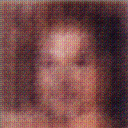
\includegraphics[width=150px]{500_fake_images/samples_5_142.png}%
\caption{A Black And White Cat Is Sitting In The Dark}%
\end{figure}

%
\end{document}